\documentclass[10pt]{article}
\usepackage[polish]{babel}
\usepackage[utf8]{inputenc}
\usepackage[T1]{fontenc}
\usepackage{amsmath}
\usepackage{amsfonts}
\usepackage{amssymb}
\usepackage[version=4]{mhchem}
\usepackage{stmaryrd}
\usepackage{graphicx}
\usepackage[export]{adjustbox}
\graphicspath{ {./images/} }

\title{5 D) \(\begin{gathered}\text { Akademia } \\ \text { Pomorska } \\ \text { w Stupsku }\end{gathered}\) }

\author{}
\date{}


\begin{document}
\maketitle
\begin{center}
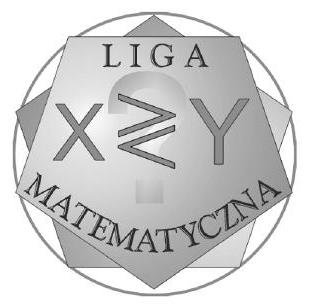
\includegraphics[max width=\textwidth]{2024_11_21_7f0a65778be44e58ebeag-1}
\end{center}

LIGA MATEMATYCZNA im. Zdzisława Matuskiego

FINAE 26 marca 2019\\
GIMNAZJUM\\
(klasa VII i VIII szkoły podstawowej, klasa III gimnazjum)

\section*{ZADANIE 1.}
Trójkąt podzielono na dwa trójkąty równoramienne i czworokąt o kącie o mierze \(80^{\circ}\) tak, jak na rysunku. Wyznacz miarę kąta \(\alpha\).\\
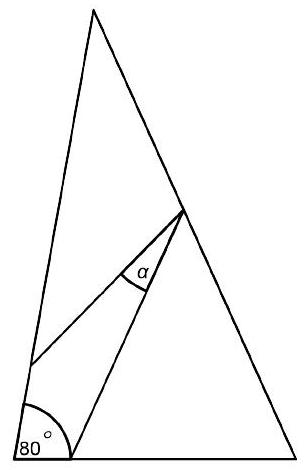
\includegraphics[max width=\textwidth, center]{2024_11_21_7f0a65778be44e58ebeag-1(1)}

\section*{ZADANIE 2.}
Ania chce zbudować sześcienną kostkę o wymiarach \(4 \times 4 \times 4\) mając 32 białe i 32 czarne sześciany jednostkowe. Planuje uzyskać na powierzchni kostki jak najwięcej białych ścian sześcianów jednostkowych. Jaka część powierzchni kostki będzie biała przy takim ustawieniu?

\section*{ZADANIE 3.}
Bartek napisał kilka dwucyfrowych liczb naturalnych mających tę własność, że każde dwie z nich są względnie pierwsze, ale żadna z nich nie jest liczbą pierwszą. Ile najwięcej liczb mógł napisać?

\section*{ZADANIE 4.}
Wyznacz wszystkie liczby całkowite dodatnie \(n\) i \(d\) o tej własności, że dzieląc liczbę 164 przez \(d\) otrzymamy iloraz \(n\) oraz reszte 10.

\section*{ZADANIE 5.}
Znajdź wszystkie liczby trzycyfrowe, które są 50 razy większe od sumy swoich cyfr.


\end{document}